\section{Application sandboxing}\label{sect:sandbox}

\begin{figure}[t!]
  \centering
  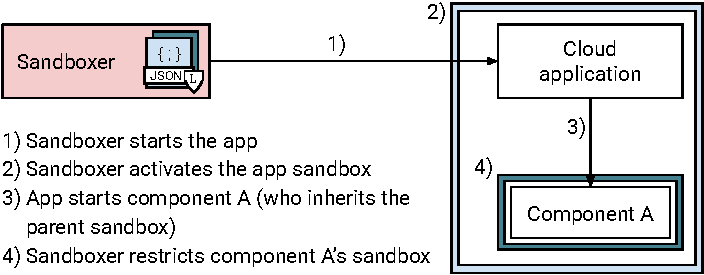
\includegraphics[width=0.8\columnwidth]{chapters/dmng/fig/landlock_overview.pdf}
  \caption{Landlock sandbox setup and inheritance}
  \label{fig:landlock}
\end{figure}

In this work we implement the sandbox leveraging Landlock, an
unprivileged sandboxing mechanism officially merged into the Linux
kernel in 2021 (version 5.13), with the goal of mitigating the
security impact of bugs and unintended or malicious behavior in
user-space application. The main reasons why Landlock was preferred to
alternative sandboxing solutions such as Google
Sandbox2~\cite{sandbox2} are: 1) it does not rely on a proxy to
implement the restrictions, hence it ensures low overhead at runtime,
and 2) it is directly implemented within the kernel, thus it provides
strong security guarantees. This section clarifies how policies are
enforced with Landlock. Furthermore, it explains how {\tt rwx} policy
rules are translated into the Landlock permission model, and how
restrictions are inherited by new components dynamically spawned at
runtime.

The sandboxer is an extension of \dmng written in Rust that receives
the JSON policy as input and modifies the application start procedure
setting the permissions available to components before they are
executed. The first task performed by the sandboxer is then to
translate the {\tt rwx} policy rules into the action-based permission
model implemented by Landlock. In detail, Landlock groups permissions
into {\em rulesets}, which collect the {\em actions} (e.g.,
FS\textunderscore EXECUTE, FS\textunderscore READ\textunderscore FILE)
permitted on each {\em object} (e.g., file, directory). The sandboxer
separates the available actions to match the {\tt rwx} categories, and
then leverages the {\em landlock\textunderscore create\textunderscore
  ruleset()} and {\em landlock\textunderscore add\textunderscore
  rule()} interfaces to populate the rulesets accordingly. To activate
the restrictions, a call to {\em landlock\textunderscore
  restrict\textunderscore self()} is perfomed. The process is
illustrated in Figure~\ref{fig:landlock}.

An important property defined by Landlock is {\em policy inheritance}.
Whenever a new component is dynamically spawned by the application in
a child process, it automatically inherits the restrictions set on the
parent. Moreover, after a ruleset has been activated, no new
permissions can be granted to a component, as the ruleset can only be
further restricted. Figure~\ref{fig:landlock} shows the policy
inheritance process for a generic application. The figure also shows
how the inherited ruleset is further narrowed with a subsequent call
to {\em landlock\textunderscore restrict\textunderscore self()} by the
component.



%%% Local Variables:
%%% mode: latex
%%% TeX-master: "../main"
%%% End:
